%% This is file `DEMO-TUDaSciPoster.tex' version 3.23 (2022/03/21),
%% it is part of
%% TUDa-CI -- Corporate Design for TU Darmstadt
%%
% !TeX program = lualatex
%%

\documentclass[
	accentcolor=3c,
%	boxstyle= boxed, % Boxen mit abgerundeten Ecken, farbigem Titelblock
	boxstyle=colored, % Boxen mit farbigen Titelblock, keine vertikalen Linien
%	boxstyle=default % Voreinstellung, ohne Farbe, ohne vertikale Linien
%	logofile=example-image, %Falls die Logo Dateien nicht vorliegen
	colorback=false,
	title=small
	]{tudasciposter}

%Sprache
\usepackage[ngerman,main=english]{babel}
\usepackage[autostyle]{csquotes}


\usepackage{multicol}
\usepackage{booktabs}
\usepackage{tabularx}
\usepackage[version=4,arrows=pgf-filled]{mhchem}
%\usepackage{mwe}
\usepackage{layouts}

\def\app#1#2{%
	\mathrel{%
		\setbox0=\hbox{$#1\sim$}%
		\setbox2=\hbox{%
			\rlap{\hbox{$#1\propto$}}%
			\lower1.1\ht0\box0%
		}%
		\raise0.25\ht2\box2%
	}%
}
\def\approxprop{\mathpalette\app\relax}


\begin{document}
	\title{Two-layered Vectorial Kernel Models \\ for Detailed Surface Kinetics using a Goal-Oriented Approach}
	\author{\underline{Felix Döppel}\inst{1,*} Tizian Wenzel\inst{2} \and Robin Herkert\inst{2} \and Bernard Haasdonk\inst{2} \and Martin Votsmeier\inst{1,3}}
	\institute{\inst{1}Technische Universität Darmstadt,  64287 Darmstadt, Germany, \hfill \inst{*}Contact: felix.doeppel@tu-darmstadt.de \\
	\inst{2}Universität Stuttgart, 70511 Stuttgart, Germany, \\
	\inst{3}Umicore AG \& Co. KG, 63457 Hanau, Germany
	}
	%\inst kann in den Autor und Institutsfeldern genutzt werden um eine Zuordnung zu ermöglichen. Bei Nummerierung ist der Nutzer dafür verantwortlich Konflikte mit \thanks zu vermeiden.
	%\titlegraphic{\includegraphics[width=.5\linewidth]{example-image}}
%	\footerqrcode{https://www.chemie.tu-darmstadt.de/votsmeier/ak_votsmeier/index.en.jsp}
	\footerqrcode{https://orcid.org/0000-0003-4733-9872}
	\footer{
		[1] D. Micale, C. Ferroni, R. Uglietti, M. Bracconi, M. Maestri, \textit{Chemie-Ingenieur-Technik} \textbf{2022}, 1–19.
		[2] Paper 1 \newline
		[2]
	}

%Instituts/Sponsorenlogos von links nach rechts
\footergraphics{
	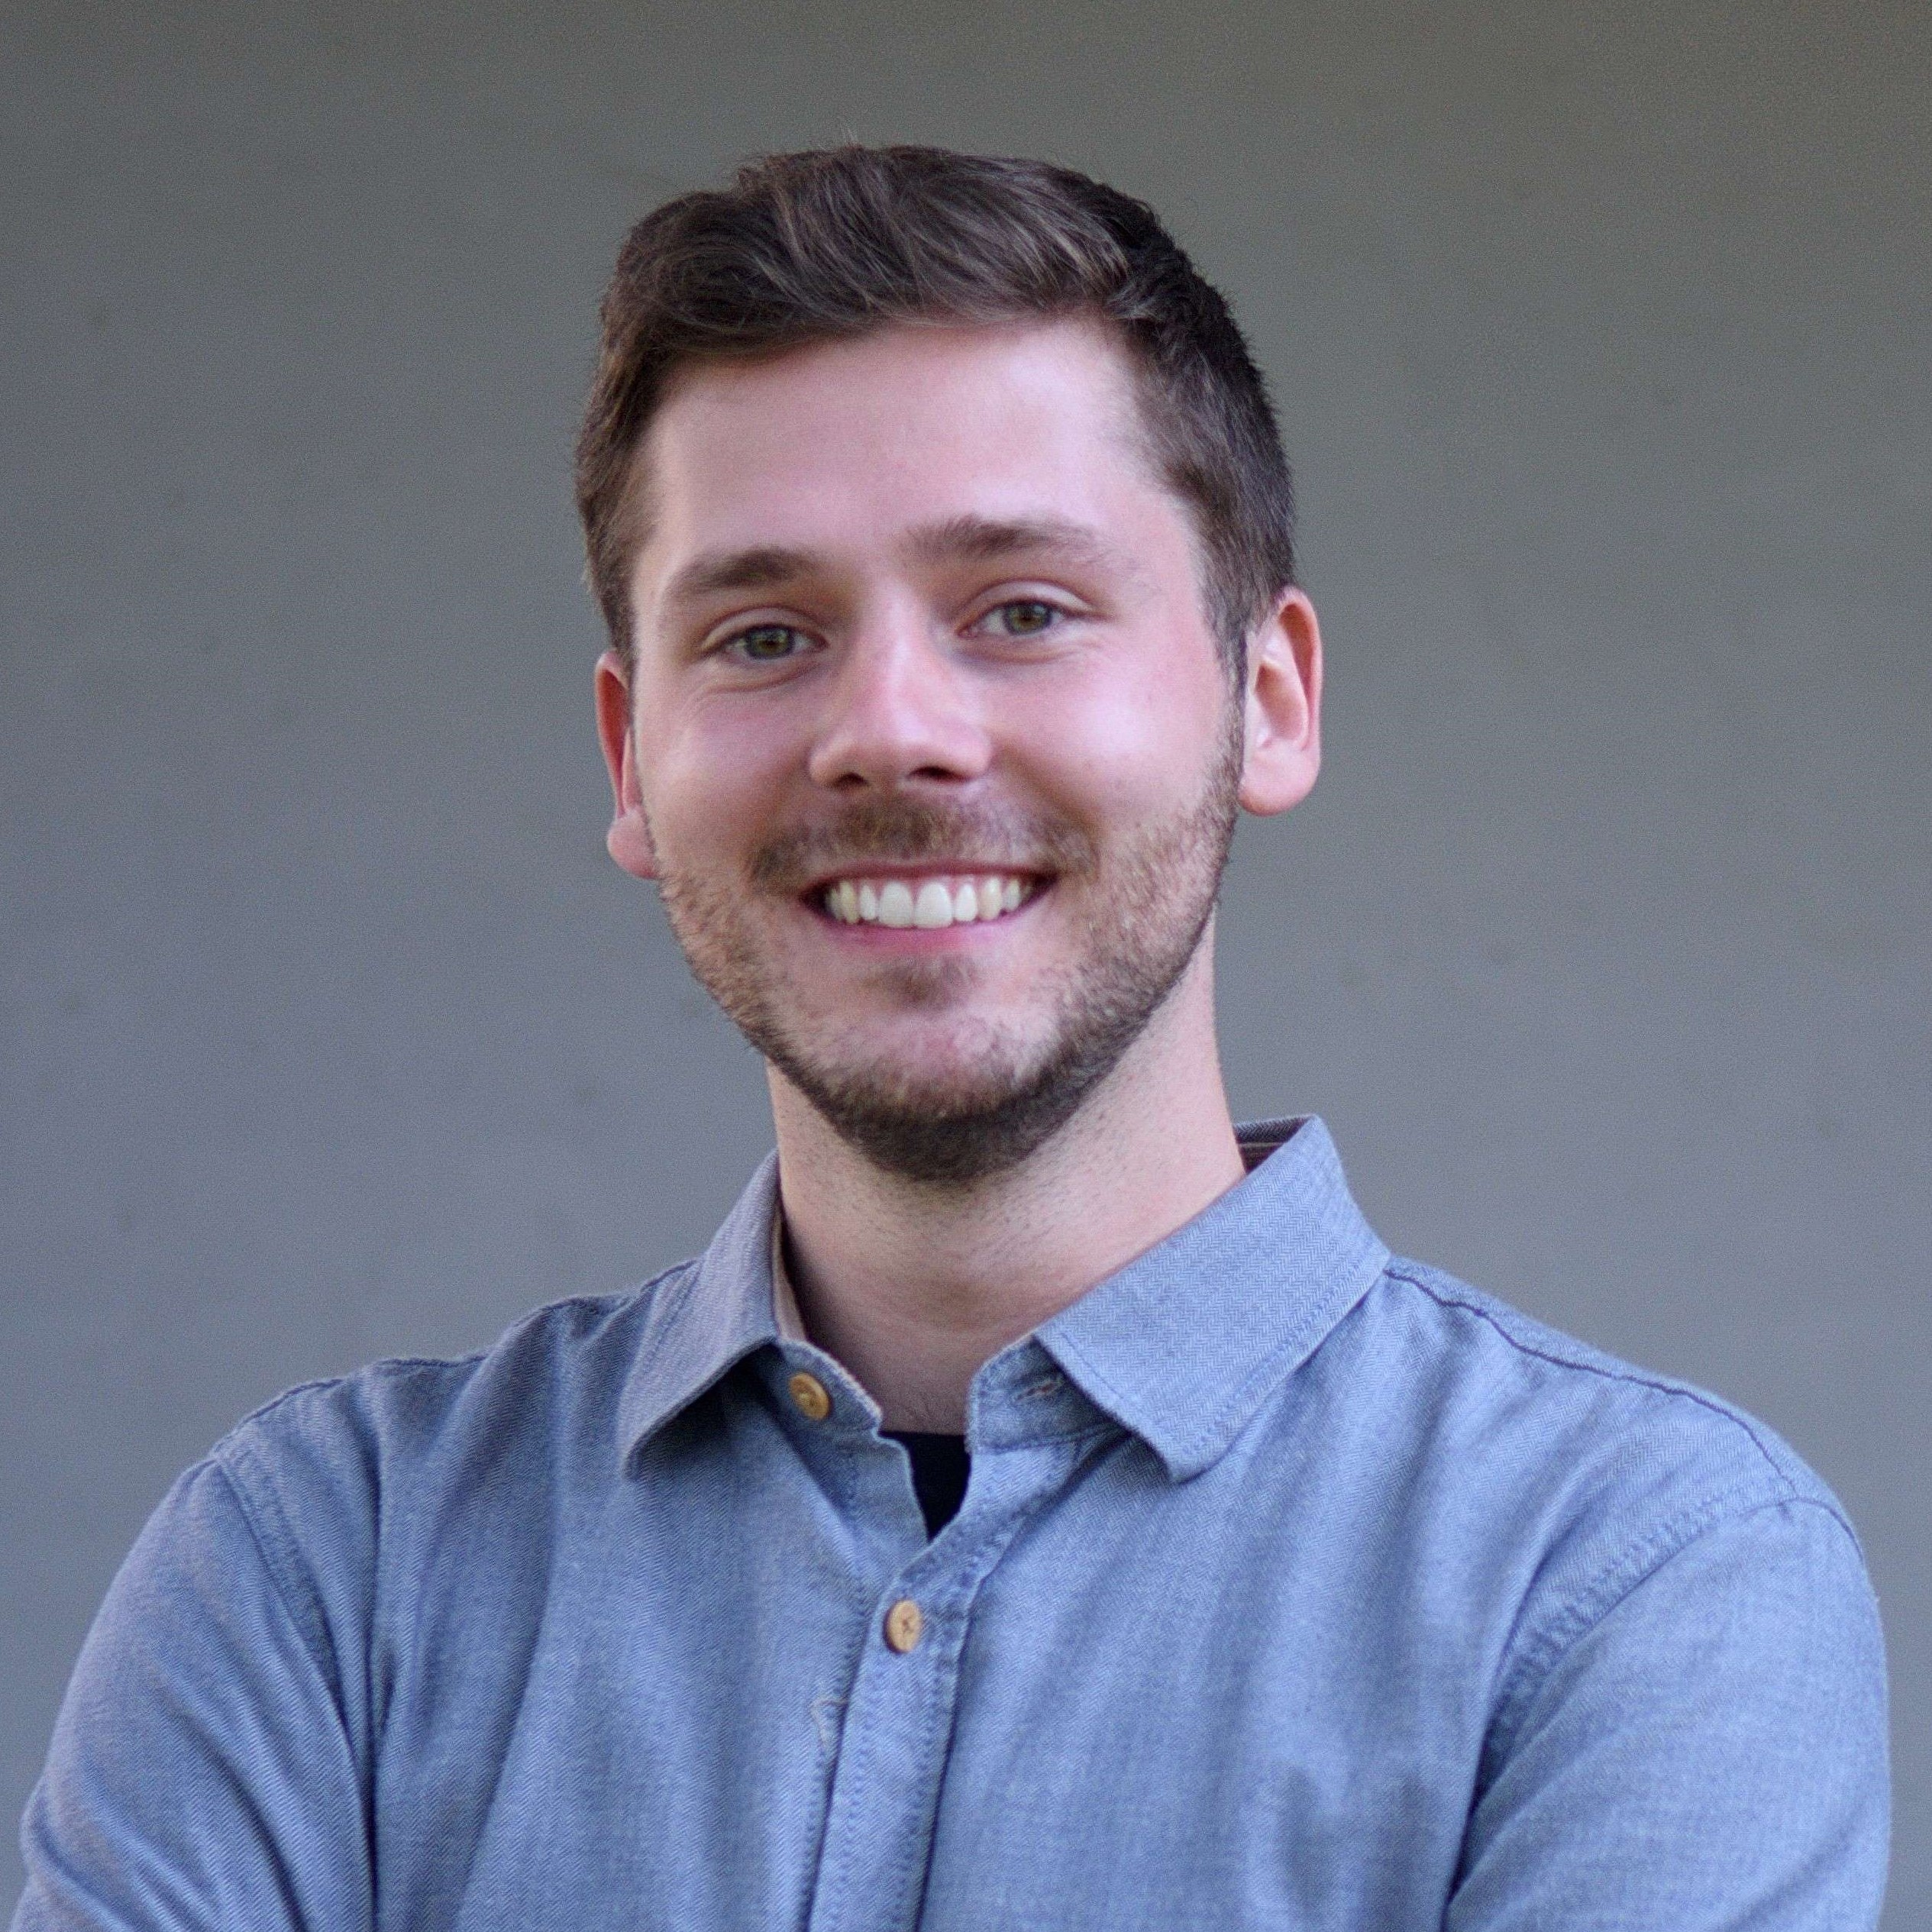
\includegraphics[height=\height]{abb/Profile_Pic_FD}
}

\begin{tcbposter}[
	poster={
		columns=8,
		rows=12,
		spacing=1cm,
%		showframe, %Gitter einblenden. Für Platzierung häufig hilfreich
	},]

\begin{posterboxenv}{name=GraphicalAbstract,column=1,row=1,span=8,rowspan=4}
%	textwidth in cm: \printinunitsof{cm}\prntlen{\textwidth}
	\centering
%	\includegraphics[width=.275\textwidth]{abb/VKOGA_scheme/VKOGA_scheme_short}
%	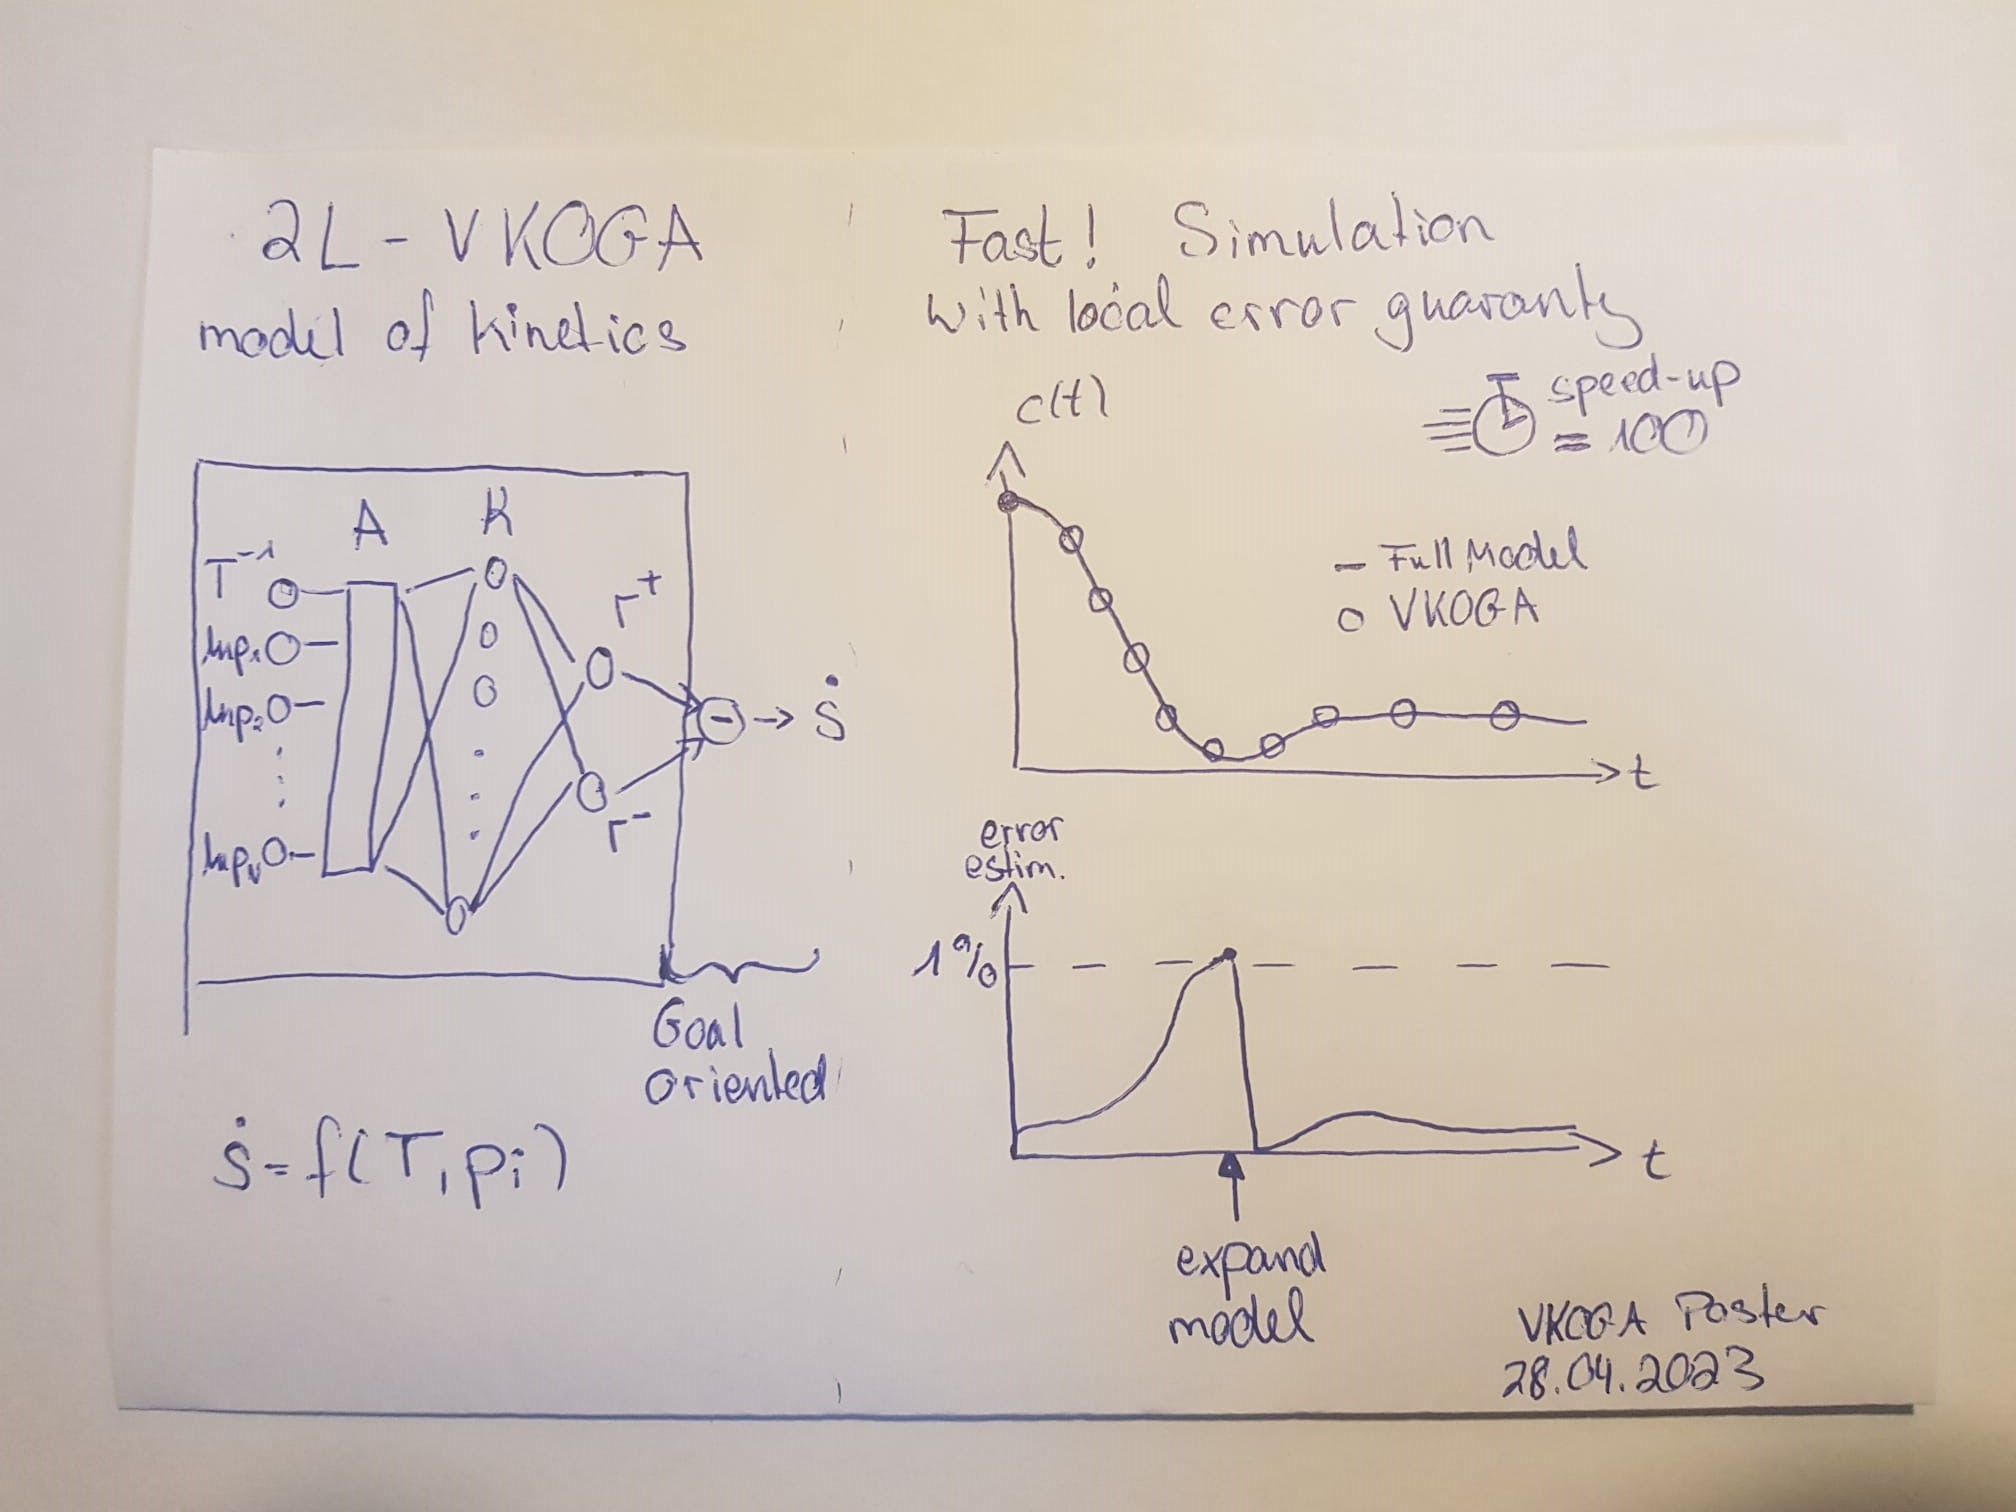
\includegraphics[width=.4\textwidth]{abb/VKOGA_Graphical_Abstract_draft.jpeg}
	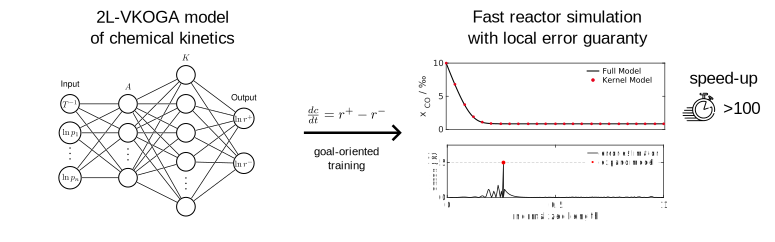
\includegraphics[width=\textwidth]{abb/GA_draft}
\end{posterboxenv}

\begin{posterboxenv}[title=1. Introduction]{name=intro,column=1,row=5,span=4,rowspan=2}
	\begin{itemize}
		\item Kinetics are the computational bottleneck in detailed reactor simulations\textsuperscript{[1]}
		\item Machine Learning surrogates speed up simulations
		\item Kernel models are deterministic and fast to train 
%		\item Goal oriented training increases data efficiency
		\item Challenge: Provide accurate surrogates with few training data
	\end{itemize}
\end{posterboxenv}

\begin{posterboxenv}[title=2. Methods]{name=Methods,column=5,row=5,span=4,rowspan=2}
	\begin{itemize}
		\item Watch a model train: QR Code to GIF of model training
		\item Model formation and consumption rates while optimizing source terms\textsuperscript{[2]}
		\item Validate in plug-flow reactor simulation
		\item Expand the model on-the-fly if error gets too high
	\end{itemize}

\end{posterboxenv}

\begin{posterboxenv}{name=Further Information,row=7,rowspan=4,column=5,span=4}
	\includegraphics[width=.485\textwidth]{abb/VKOGA_error} %{example-image-a}
	\includegraphics[width=.485\textwidth]{abb/VKOGA_hist}
	%	\captionof{figure}{Histogram.}
	\captionof{figure}{Prediction error vs. number of selected centers for standard and goal oriented approach.}
\end{posterboxenv}

\begin{posterboxenv}[title=3. Results]{name=Results,column=1,row=7,span=4,rowspan=4}
	\begin{itemize}
		\item Goal oriented training increases data efficiency
		\item Data utilization can be chemically understood
		\item Built in error estimator provides guaranty for local accuracy
		\item Reactor simulations are 
		\item Models can be trained on-the-fly, even with zero previous training
	\end{itemize}
	\vspace{2cm}
	\captionof{table}{Advantages of using VKOGA instead of Neural Networks}
	\begin{tabularx}{\textwidth}{XX}
		\toprule
		Pro & Contra \\ \midrule
		fast training & less accurate \\ 
		very data efficient & fewer libraries/literature available\\
		internal error estimator & no GPU implementation\\		
		\bottomrule
	\end{tabularx}%
	


\end{posterboxenv}

\begin{posterboxenv}[title=4. Conclusion]{name=Conclusion,column=1,row=11,span=8,rowspan=2}
\begin{multicols}{2}		
	\begin{itemize}
		\item Speed up reactor simulations by factor >100
		\item Precision guaranty due to internal error estimator
		\item Goal oriented approach reduces demand for data
	\end{itemize}
\end{multicols}

\end{posterboxenv}

\end{tcbposter}

\end{document}


